This chapter describes the steps followed for a performance analysis of FastJet. Initially the installation process on the two computing systems, Cirrus and ARCHER is discussed, followed by the set-up of the analysis framework. Then, the profiling process is explained and the results are examined. Finally, the last section of this chapter looks into some efforts that were made to speed-up FastJet and what the future may hold for it.

\section{FastJet on different Computing systems}
For the needs of this project, FastJet was installed on two computing systems, Cirrus and ARCHER. This section provides some basic information regarding those systems, and also any abnormalities in the process of installing FastJet on them.
\subsection{Cirrus}\label{ch:cirrus}
Cirrus was the main system that performance experiments were run on and it was selected for a number of reasons. It has modern Intel processors, provides the ability to choose between two compilers (GCC and Intel), allows for easy testing on the front-end but also for exclusive access to back-end nodes via the batch system, the software system is fairly standard Linux, and the student was already familiar with it from the MSc courses. 

\subsubsection{Hardware}
Cirrus\cite{cirrus} was the main system that the analysis for FastJet was performed on. It is one of the EPSRC Tier-2 National HPC Services and consists of 280 compute nodes, each with 256 GB of memory, connected together by a single Infiniband fabric. Each node contains two 2.1 GHz, 18-core Intel Xeon processors. In total there are 10.080 cores in Cirrus. Since Cirrus' processors support hyperthreading, up to 72 cores can be used in a single node.
\subsubsection{Installation process}
The installation process on Cirrus was already included in subsection \ref{ch:fjtech} of chapter \nameref{ch:fastjet}. The reason for that is to provide a more pedagogical approach for FastJet to the reader. 

\subsection{ARCHER}\label{ch:fj-ARCHER}
The main motivation for using ARCHER was the availability of CrayPAT (which is discussed in section \ref{ch:craypat}). ARCHER, having three compilers (.,.,.) was more appealing for some performance tests, but its CPUs are older and it is it is rather non-standard in terms of the OS and setup.



\subsubsection{Hardware}
ARCHER \cite{ARCHER} is the UK National Supercomputing Service. It consists of 4920 compute nodes, each with 64 (a few nodes have 128) GB of memory. Each node contains two 12-core Intel Ivy Bridge series processors. In total there are 118.080 processing cores on ARCHER.

\subsubsection{Installation process}
ARCHER, being a CRAY machine, seemed like a good option in order to profile FastJet using CrayPat. Installing FastJet on ARCHER with the GNU compiler (which is the default FastJet compiler), ran smoothly. In order to use CrayPat for profiling though, the code in question should be compiled using the Cray compiler. As a result, an effort was made to install FastJet again, but this time, when executing the configure file, the Cray Compiler was chosen (PrgEnv-cray module is required in order to use the Cray compiler but it is loaded by default on ARCHER):

\begin{lstlisting}
./configure CC=cc CXX=CC --prefix=$PWD/../fastjet-install
make
\end{lstlisting}

A number of GNU compiler flags are hard-coded into the compiling process. These flags are incompatible with the Cray compiler, and caused the compilation to fail.  As a workaround, the Cray wrapper on top of GNU compiler was used, so that the compiler flags would be compatible:
\begin{lstlisting}
module swap PrgEnv-cray PrgEnv-gnu

./configure --prefix=$PWD/../fastjet-install
make
\end{lstlisting}

On ARCHER every library is by default linked statically. As it turns out, some of FastJet libraries cannot be linked statically and caused the compilation to fail. From ARCHER documentation, a way to link libraries in a dynamic way was tried: 

\begin{lstlisting}
./configure CC=cc CXX=CC CRAYPE_LINK_TYPE=dynamic --prefix=$PWD/../fastjet-install
\end{lstlisting}

This still produced errors, and the compilation failed. At this point, considering that ARCHER was not the main system to be used for the dissertation project, it was decided to stop the effort and focus the performance analysis using Cirrus.

\section{Setting up the analysis}
\subsection{Choice of algorithms}
As described in the previous chapter, FastJet provides the opportunity to perform several different types of analysis. Naturally, for the scope and length of this project, it seemed sensible to make a selection of a few of them. Therefore, two jet reconstruction algorithms (chapter \ref{ch:seq_alg}), Cambridge/Aachen and the anti-$k_t$, were chosen to perform the analysis on. The decision for these two algorithms was based on the fact that they are considered the best on jet clustering by the physics department of the university of Edinburgh, are widely used, and any possible performance improvement on them would have a considerable impact on the community. 


\subsection{Choice of input data}
Having chosen the algorithms, it was then time to find appropriate and meaningful input data. 

A large input file consisting of sixty thousand particle collision events, and a size of 220MB, was supplied by the particle physics department for the needs of the project. Every event consists of around 100 particles. Particles per event is an important parameter for the reconstruction and it greatly affects the algorithmic strategy of FastJet.

\subsection{Writing the test code}\label{ch:testcode}
For the purpose of the project a C++ program was written, utilising FastJet's classes and algorithms, in order to analyse their performance. The program was separated in three main functions:
\begin{itemize}
    \item \textbf{read input data:} Stores all the particles per event in a vector of pseudojets.    
    \item \textbf{perform clustering:}
    Loops through all the events, and for each one of them, performs the jet reconstruction according to the parameters set.
    \item \textbf{print reconstructed jets:}
    Prints to the screen all the reconstructed data.
\end{itemize}

The writing of the program was greatly aided and influenced by the provided FastJet examples; nevertheless some considerable work had to be done to tailor it for the needs of the project. The test code in its entirety can be found in Appendix \ref{ch:test_code_code}. 

\subsection{Performance analysis framework}
At several different points of the analysis, changes were attempted to the default behaviour of FastJet either to deepen the understanding of the software or to check a speculation. These changes could be different compiler flags, different compilers, altering the test code, or even modifying the FastJet libraries. Usually, each change was followed by measuring the performance of FastJet under the new conditions.

To make sure that the right results were still produced after each modification, a reference output file containing the correct results was created. After each run, the newly created output file was compared to the reference output file. In some occasions, changes would create an output file different to the reference output file, while still being correct; for example the jets would just be out of order. Those were treated separately.

Every performance measurement, unless explicitly stated otherwise, was run on the back-end of Cirrus and is the average of at least 5 runs. To achieve accuracy of the timing measurements, c++11's class std::chrono was used. Finally on\textbf{}ly the time spent in the perform function was timed. This is because, the time spent during IO is not relevant to the scope of the project.



\section{Choice of compiler and compiler optimisation flag}

After getting FastJet up and running, writing a test case, and getting the input data, some initial tests were run in order to gain a basic understanding of FastJet's performance.

Cirrus has two compilers installed, GNU and Intel. FastJet and the test code were compiled with each one of the compilers (GNU version  4.8.5, Intel 17) and optimisation flag (O0, O1, O2, O3, Ofast\footnote{Flag -Ofast enables all optimisation of O3, and also lets the compiler ignore finite precision of floating point numbers. This allows more optimizations, but can cause inaccuracies in the results due to rounding errors.}).

The process was repeated for two algorithms, anti-$k_t$ and Cambridge. The results can be seen in figure \ref{fig:flags}. The performance of both compilers for both algorithms is almost identical, although the GNU compiler performs slightly better. There is a big improvement between the first two compiler optimisation flags, and optimisation flag O2 performs better than O3. The reason for that may be that O3 flag optimizations increase code size (for example more aggressive loop unrolling), which can sometimes lead to slower performance. 


\begin{figure}[H]
    \centering
        \begin{subfigure}[b]{0.3\textwidth}
        \centering
    \end{subfigure}
    \hfill
    \begin{subfigure}[b]{0.3\textwidth}
        \centering
        
\includegraphics[width=0.6\textwidth]{images/flagsleg.eps}
    \end{subfigure}
    \hfill
    \begin{subfigure}[b]{0.3\textwidth}
    \centering
    \end{subfigure}
    
    \begin{subfigure}[b]{0.48\textwidth}
        \centering
        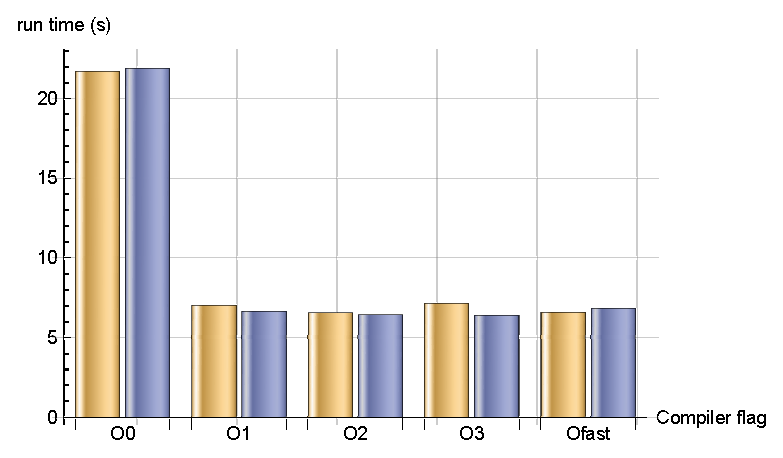
\includegraphics[width=1.2\textwidth]{images/flagskt.eps}
        \caption{Anti-$k_t$}
    \end{subfigure}
    \hfill
    \begin{subfigure}[b]{0.48\textwidth}
        \centering
        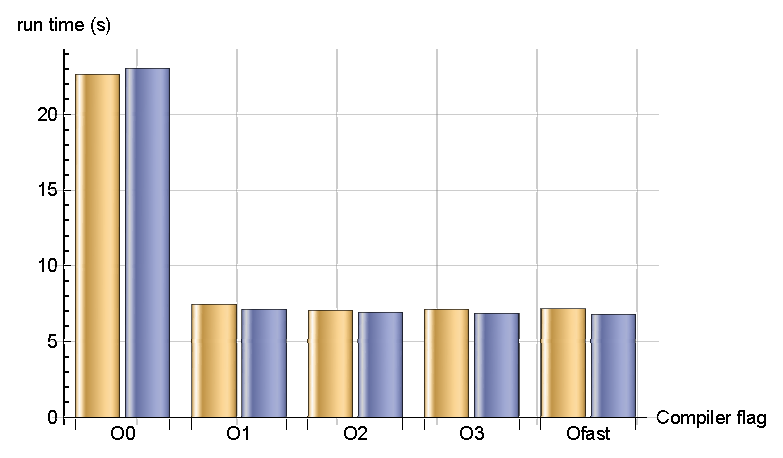
\includegraphics[width=1.2\textwidth]{images/flagscam.eps}
        \caption{Cambridge}
    \end{subfigure}
    \hfill
    \caption{Run-time versus compiler optimisation flag for two compilers. Each plot represents a different algorithm}
    \label{fig:flags}
\end{figure}

\section{Finding the most suitable profiler}
Profiling is the process of measuring an application or system. Profiling tools can provide information for different parts of the application: functions call, memory usage, CPU load, and resource usage. Two types of profiling that are worth mentioning are statistical profiling and tracing. Statistical Profiling is a way to profile an application by taking samples of the execution state during regular intervals at run-time. Tracing tools on the other hand generate results based on a detailed log of events within the program.

The initial experiments described in the previous section, provided an idea of FastJet's performance. The next step was to pinpoint which of the numerous FastJet functions are called with the current choice of algorithms, number of particles per event, and radius R. Afterwards, inspect which lines of code and loops are the most computationally expensive. 

\subsection{GNU gprof}

GNU Gprof is a statistical profiler for Unix based applications. Usually, the simplicity of usage it offers, makes it the fist choice when profiling software. GNU gprof version 2.25 which is installed on Cirrus was used. As per the usage instructions, FastJet software and the test code were compiled with the -pg flag. 

Interestingly, the profiling result only accounted for a small fraction of run-time. Only the time spent in the test code, but not in any FastJet functions, was accounted for. After seeking advice from the relevant gprof documentation, it was realised that GNU gprof cannot profile libraries that are linked dynamically. 

From Cirrus documentation, the command ldd + <executable> was used to check which libraries were linked dynamically. Indeed, a number of FastJet objects showed up as being linked dynamically. The -Bstatic flag followed by the full path of those libraries was used when compiling to force a static linking.

This time, the result of gprof accounted for the whole run-time and the FastJet functions explicitly called by the test code were shown. Nevertheless, profiling did not show the percentage of time spent in any other internal functions of FastJet. It was then decided that it was better, in terms of time-management and to keep to the right track for the project, to try and use a different profiler.


\subsection{CrayPat}\label{ch:craypat}
The Cray Performance Measurement and Analysis Tools (CrayPat) are a suite of utilities that capture and analyse performance data generated during the execution of a program on a Cray system\cite{craypat}. It can be used for both statistical profiling and tracing. CrayPAT is a very powerful tool that is well documented and frequently used by EPCC staff. It seemed to be a good candidate to provide insights on FastJet at the time. 

CrayPat requires that the source code is compiled using the Cray compiler on a Cray machine in order to succeed in profiling the software. However, as discussed on subsection \ref{ch:fj-ARCHER}, a number of difficulties arose while trying to install FastJet on ARCHER with the Cray Compiler. As a result, it proved more time consuming than intended to get any profiling results using CrayPat. Once more, to save time, it was decided to choose a different profiler.

\subsection{Gperftools}
A good alternative to the previous profilers was the gperftools profiler\cite{gperf}, a set of tools for statistical performance profiling and memory checking. Although, again, the profiling process was not trouble-free, the results were satisfactory. 

As gperf tools profiler is not currently installed on Cirrus and due to the limited privileges of the student's account, there was not a straightforward way to install in. As a result, it was installed in a Singularity container and copied to Cirrus. 

\subsubsection{Creating a singularity container image}\label{ch:singularity}
A container image is a lightweight, standalone, executable package of software that includes everything needed to run an application: code, runtime, system tools, system libraries and settings. Conveniently, Singularity\cite{kurtzer2017singularity}, a type of container, is already installed on Cirrus. 

First of all, one has to create the singularity image on a system with administrative privileges, through a singularity recipe. The student's laptop was chosen for that purpose. A singularity recipe is a text file, containing the necessary information for the image to be built. A singularity recipe was created, greatly influenced by the singularity documentation.

\lstinputlisting[language=bash]{codes/singularity_recipe.sh}

In order to create the image, the following command was executed.

\begin{lstlisting}[language=bash]
sudo singularity build --writable image_name.sing recipe.def
\end{lstlisting}

Where, the flag --writable provides the possibility for the image to be changed in a later time. The next step was to copy the newly created image to Cirrus. Having done that, the following command initiates an interactive shell inside the image, allowing the the software installed in it to be used.

\begin{lstlisting}[language=bash]
module load singularity
singularity shell image_name.sing
\end{lstlisting}

\subsubsection{Profiling}\label{ch:gerf1}
There exist two main ways to profile software with gperf tools. Both are just different alternatives of starting the profiler before the executable to be profiled. The first option is to recompile FastJet and the test code with the flag -lprofiler, and the second to set the environmental variable LD\_PRELOAD accordingly. Bellow, the second method, which was followed, is explained. The environmental variable CPUPROFILE is set to be the output file of the profiling.

The process to follow in order to profile the code on Cirrus is: 
\begin{lstlisting}[language=bash]
module load singularity
singularity shell <path_to_the_singularity_image> #Enter an interactive shell where gperf tools are installed

#LD_PRELOAD allows the profiler to be executed prior to the software
#CPUPROFILE sets the output file of the profiling
LD_PRELOAD=/usr/lib/libprofiler.so CPUPROFILE=./profiling_result.prof ./<path_to_executable> #in one command
\end{lstlisting}

After that, the profiling of the software will start. Upon completion, a terminal output will read:  PROFILE: interrupts/evictions/bytes = \textit{"some number"}\\ An output file will be created to where CPUPROFILE is pointing at. 

\subsubsection{Processing the output}

The output file from the profiling, can be used in order to create more human readable profiling results. The command to do that is:
\begin{lstlisting}[language=bash]
google-pprof [Output Type] [Granularity] [Display] ./profiling_result.prof > output.file
\end{lstlisting}

where:
\begin{itemize}
    \item \textbf{Output} denotes the output file type (text, pdf, gif, etc)
    \item \textbf{Granularity} is what nodes will represent (addresses, lines, functions, files)
    \item \textbf{Display} provides a few possibilities on the nodes are shown.
\end{itemize}

For example a user friendly output saved as pdf (similar to the one shown in figure \ref{fig:gperfnatikt}) can be requested by using:
\begin{lstlisting}[language=bash]
google-pprof --pdf --functions ./profiling_result.prof
    > output_file.pdf
\end{lstlisting}

\subsubsection{Focused profiling}
The profiling process described until now, accounts for the whole run-time of the software. As this project focuses only on the clustering phase, a way was sought for selective profiling. Two ways were found.

The first one involved, making use of calls from the test code to the functions ProfilerStart() and  ProfilerStop(). For this to work out, the profiling was stopped at the start of the main function, started again right before the clustering function and stopped again afterwards. The header file <gperftools/profiler.h> has to also be included for the functions to work. 

The reader may have noticed that the contents of the singularity recipe file include the installation the GNU compilers. This is only necessary for the method that has just been described. The reason is that, once the header file of the previous paragraph is included in the source code, gperf tools must be installed on a system for the code to compile. Thus, the interactive shell is loaded prior to compiling.

The second way for selective profiling is much simpler, but was discovered a while after the first one. It involves profiling the whole run-time of the software and then using the clause \verb|--|focus=<desired\_function> while processing the output. This only performs the analysis for the <desired\_function>. There exist also the \verb|--|ignore clause with the opposite functionality.

\subsubsection{Profiling results} 
The profiling result of gperf tools was very informative. FastJet internal function calls are shown very clearly. The graph for the anti-kt and the Cambridge algorithms, focused only on the perform\_clustering function, can be seen on figures \ref{fig:gperfnatikt} and \ref{fig:gperfcamb} respectively. Each node represents a procedure. The directed edges indicate caller to callee relations. Each node is formatted as follows: class name, function name, local percentage, cumulative percentage.

\begin{figure}[H]
    \centering
\includegraphics[width=1\linewidth]{august2_antikt.jpeg}
    \caption{Profiling result using gperf tools for the anti-kt algorithm, focused only on the perform\_clustering function.}
    \label{fig:gperfnatikt}
\end{figure}

\begin{figure}[H]
    \centering
\includegraphics[width=1\linewidth]{images/august2_camb.jpg}
    \caption{Profiling results for the Cambridge algorithm, focused only on the perform\_clustering function.}
    \label{fig:gperfcamb}
\end{figure}

\subsubsection{Discussion} 
Looking at the results, it is clear that both the Cambridge and the anti-$k_t$ reconstruction algorithms make substantial calls to a function called ClusterSequence\_TiledN2. That is the function that calculates the smallest distance between any two particles, as has been discussed on section \ref{ch:seq}. It can also be deduced that the tiled strategy is chosen. FastJet tiled strategy is explained on subsection \ref{ch:tiled}.

A closer look at the code of the computationally expensive function revealed that it consists of a number of loops. The next chosen step was to find which of those loops were the most computationally expensive in that function.

Going back to the output processing with pprof, this time  \verb|--|lines was selected as granularity option. Unfortunately it didn't produce sensible results, as in the output file, there were question marks instead of line numbers. 

In order to solve that, two attempts were made. The first involved compiling the whole software (FastJet libraries and test code) with the -g flag, so that full debugging information would be produced or without any compiler optimisations (O0 flag). For the second attempt, the alternative profiling way of the two discussed on subsection \ref{ch:gerf1} was tried. Neither of them improved the outcome.

Although gperf tools profiler succeeded in pointing out the most expensive function, it was thought better to try another profiler, hoping it would be able to provide line by line results.

\subsection{Intel VTune Performance Analyzer}\label{ch:vtune}
The next choice of profiler was Intel VTune Performance Analyzer\cite{malladi2009using}, a commercial application for software performance analysis, whose goal is to detect performance bottlenecks in an application. Version 17 is already installed on Cirrus. FastJet was installed again using the Intel compiler.

Using the graphical user interface provided by the profiler, a  new analysis was initiated pointing to the executable, and basic hotspots analysis was chosen as a good starting point for the algorithm analysis.

The results were thorough and informative. For example, using the top-down tree tab shows the most computationally expensive functions in descending order. Filtering in on the perform\_clustering function produces the result of figure \ref{fig:vtune1}. The results are in agreement with the previous output of gperf tools. Again, it can be seen that the biggest portion of run-time is spent on the Cluster\_Sequence\_Tiled\_N2 function.

VTune Amplifier is also able to provides the option to show the source code along with information on the percentage of run-time spent in each line. Figure \ref{fig:vtune2} illustrates that. 

\begin{figure}[H]
    \centering
    \includegraphics[width=0.9\textwidth]{images/vtune1.JPG}
    \caption{Most computationally expensive functions, from VTune. The results have been filtered in on perform\_clustering function. It can be seen that the most time is spend on the Clsuter\_Sequence\_TiledN2 function.}
    \label{fig:vtune1}
\end{figure}

\begin{figure}[H]
    \centering
    \includegraphics[width=0.85\textwidth]{images/vtune2.JPG}
    \caption{Example result from VTune showing the percentage of run-time spent in each line of source code.}
    \label{fig:vtune2}
\end{figure}

Using the above information, two loops, accounting for 14.2\% (listing \ref{lst:bigishloop}) and 33.3\% (listing \ref{lst:bigloop}) of the clustering time respectively, were pinpointed. Discussion for these loops takes place in the next section.


\section{Discussion of Profiling results}\label{ch:proftalk}
The profiling process revealed that a function called Cluster\_Sequence\_TiledN2, utilising the tiled strategy discussed in section \ref{ch:tiled}, is responsible for the largest proportion of run-time. In it,two loops were identified as the most computationally expensive, accounting for 14.2\% and 33.3\% of the clustering time.

The first of the two most computationally expensive loops is performing part of the set-up for the tiled strategy, and can be seen in listing \ref{lst:bigishloop}.  It loops through all tiles. For every tile, it calculates the nearest neighbour (NN) and nearest neighbour's distance (NN\_dist) of every jet(pseudojet) in the current tile and all tiles to the right side (RH) of it. 

 For each pair of jets processed, the algorithm checks whether the second jet is the nearest neighbour of the first one and whether the first jet is the nearest neighbour of the second. As a result the tiles to the left of each tile do not have to be looped through as they have already been checked.

The second one is responsible for finding the two (developing) jets closest to each other, and is shown in listing \ref{lst:bigloop}. It takes place multiple times per event reconstruction: once per step, until all the particles have been clustered or a stopping criterion has been reached. There are four nested loops. Through every tile, every jet in that tile, all neighbouring tiles, all jets in those tiles. All newly computed distances between jets are registered, and if any of them is smaller than the registered smallest distance, the latter is updated.

For a reminder of what the clustering algorithm calling these two loops does, refer back in sections \ref{ch:seq}, \ref{ch:fjstrategy} and \ref{ch:tiled}. The number of tiles is different for each event, but the average number of tiles that the jets are being separeted into is ten.

\lstinputlisting[language=C++, caption=The second most computationally expensive loop identified that accounts for 14.2 percent of runtime.,label=lst:bigishloop,escapechar=|]{codes/bigish_loop.cc}

\lstinputlisting[language=C++, caption=The most computationally expensive loop identified that accounts for 33.3 percent of runtime.,label=lst:bigloop,escapechar=|]{codes/big_loop.cc}

At that point of the dissertation project, a number of questions were raised. Can those loops be paralelised using OpenMP? If yes, will that aid performance? With some back of the envelope calculations: analysis of each event takes around 100 microseconds. The OpenMP overhead to open a parallel region is between the range of 10-100 microseconds, depending on the system. Things are already not looking too bright in this path.

\section{Efforts to speed-up FastJet}

\subsection{Parallelise over particle events}
Each particle collision event can be worked on individually from the rest. In principle, parallelising over events, providing the workload is enough, should have a near optimal speed-up curve, relative to the number of cores. It was decided that it was worth testing this speculation. To parallelise over events in the test code the loop that calls the Cluster Sequence function was included in a parallel for loop, as can be seen on listing \ref{lst:par_events}.

\begin{lstlisting}[language=c++,caption=Code fraction that parallelised over events,label=lst:par_events,escapechar=|]
int number_of_events = all_events.size();
all_jets.resize(number_of_events);//resize the vector of vectors prior to the loop, so that the reconstructed jets will be placed in the same position as in the serial program.

#pragma omp parallel for schedule(static)
//workload is on average the same for each particle event
//Static scheduling, to avoid the overhead of sharing the workload in an other way
    for(int k=0;k<number_of_events;k++)
    {
        vector <PseudoJet> current_event = all_events[k];

        //for each event run the jet clustering 
        //with the appropriate jet definition        
        ClusterSequence clust_seq(current_event, jet_def);

        //Sort the particles in the jet from larger to smaller momentum.
        //ptmin is the threashold  momentum of particles to filter out of the jet.
        double ptmin = 0;
        vector<PseudoJet> jets = sorted_by_pt(clust_seq.inclusive_jets(ptmin));
        //save the newly reconstructed and sorted jet to the appropriate position fo the vector of vectors
        all_jets[k] = jets;
    }//end of the loop through all events
}
\end{lstlisting}

A subtle point was the sequence in which the reconstructed jets would be saved to the vector. While the output result could still be correct if the jets were stored out of sequence, there was not a way to be certain. Thus, the vector was resized to the appropriate size prior to the loop, and then each thread positioned the reconstructed  jet in the appropriate place.

A static scheduling option was chosen because all the events to be reconstructed needed on average the same computational work. There was no need for a more sophisticated scheduling option that would add extra overhead.

\begin{figure}[H]
    \centering
    \begin{subfigure}{\textwidth}
        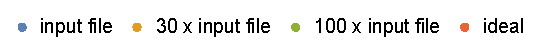
\includegraphics[width=1\linewidth]{images/coarseplotlegend.eps}
    \end{subfigure}
    
    \begin{subfigure}{\textwidth}
        \includegraphics[width=1\linewidth]{images/coarseplot.eps}
    \end{subfigure}
    \caption{fix me: coarse}
    \label{fig:coarse}
\end{figure}

To test the weak scaling, two bigger input files were created, 30 and 100 times the size of input file. Figure \ref{fig:coarse} illustrates the speed-up curve for a different number of threads for the three input files and the ideal speed-up. The bigger the input file, the better the performance, so it can be concluded that workload is the bottleneck for scaling.

\subsection{Parallelising sequential clustering algorithms}

\subsubsection{Pre-existing work}\label{ch:otherswork}

Before proceeding to the work done by the student, in parallelising the clustering algorithms category, it is worth discussing a similar work, performed in \cite{forster2017parallel}. The authors claimed to have succeeded in parallelising the kt algorithm, one of the sequential clustering algorithms used in this project.

After inspecting the work, it was realised that the authors were referring to a non-tiled, obsolete, strategy of the kt algorithm. Although a good starting point, this algorithm has no use in practice, and thus any speed-up gained relative to it has no application. The approach followed was very simplistic, attempting to provide an explanation of the parallelisation process, towards Physicists without a high performance computing background.

Nevertheless, the conclusion of the authors was that, even though the overhead of starting the OpenMP parallel region is bigger than the analysis time for each event, some speed-up was managed to be gained by utilising a thread pool; generating the worker threads only once at the start of the application. That way, the overhead of starting and stopping the threads was minimised.

\subsubsection{Work done by the student}

Following the discussion of section \ref{ch:proftalk}, an attempt to parallelise the most computationally expensive loop (shown in listing \ref{lst:bigloop}) was made. The code fragment was studied to determined any parts of it prone to race conditions. For every pair of jets being looped through, their distance is being calculated locally. This distance is then checked again the global value of the nearest neighbour of the active jet. This part, extending from line \ref{line:crit1start} to \ref{line:crit1end} was put in a critical region.

The whole loop was included in a parallel for with static scheduling clause. The reason the static scheduling was chosen was that, each event requires the same amount of work on average; the extra complexity of a more sophisticated scheduling clause was not needed. Executing the software in parallel produced the correct results but, unsurprisingly, it was much slower than serial. 

Two possible reasons were thought as candidates for the poor performance. The first is that possibly the the critical region is too restrictive. If that is the case, maybe a restructuring of the loop to allow more of the work to be performed out of the parallel region could aid performance. 

The second possible reason is that the overhead of parallelisation is bigger than the performance gain from sharing the workload.

To test the effect of the critical region on performance, the code was run in parallel without it. The output results, as expected, were wrong. Interestingly the run-time only improved slightly, but was still much slower than serial. The critical region is not the major bottleneck in parallelising FastJet; the overhead of parallelisation is.

\subsubsection{Thread pool}
Since the overhead of opening the parallel region has been identified as the major bottleneck, and following the conclusions of subsection \ref{ch:otherswork}, maybe a good idea would be to create a thread pool. This way the overhead of starting and stopping the OpenMP threads would be minimised. Unfortunately during the current work, there was not enough time to test that hypothesis, and will be left for the future.

Also, the openMP is smart enough to do it by itself. Maybe it is tricked though.

